\chapter{Analyse und Auswertung}
Um zu analysieren, wie sich die Webanwendung unter Last verhält, werden verschiedene Aspekte, wie die Netzwerkauslastung und der notwendige Arbeitsspeicher, betrachtet.

\section{Geolocations: zeitliches vs. konditionelles Update}
Bei der Aktualisierung der eigenen Position gibt es zwei Möglichkeiten diese abzufragen:

\begin{enumerate}
	\item Zeitliches Intervall definieren, in dem die Position aktualisiert wird
	\item Überwachung des Standortes über HTML5-eigene Module
\end{enumerate}

\paragraph{Intervall}
Zuerst wurde ein Intervall von 10 Sekunden benutzt, um die Positionsinformationen zu erfragen, verarbeiten und an den Server zu schicken. Das ist eine einfache Lösung, die zum gewünschten Ergebnis führt, allerdings nicht wirklich in Echtzeit abläuft.

\paragraph{watchPosition()}
Die zweite Methode ist der Abruf einer Funktion, die von der navigator-Klasse bereitgestellt wird. Mit \emph{watchPosition()} wird die Position des Gerätes überwacht und bei Veränderung eine \emph{successCallback}-Funktion aufgerufen \cite{geolocationapi}. Diese Callback-Funktion verarbeitet die aktuelle Position in einem JSON-Objekt, wandelt es in einen String um und schickt anschließend das Update an den WS Server.\\
Da watchPosition() nur auf Änderung des Standortes reagiert, können Zugriffe auf das GPS Modul des Endgeräts und damit auch der Stromverbrauch verringert werden. Daher ist diese Methode vorzuziehen und wird in der Meißner App verwendet.

\section{Webserver mit Apache2}
Hier werden die Zugriffszeiten der Anwendung gemessen. Dabei werden eine leere cakePHP Anwendung, die Loginseite der Meißner App sowie 3 Veranstaltungen mit unterschiedlichen Anzahlen von Einträgen miteinander verglichen.\\
Die Loginseite wird verwendet, da sie eine Seite mit minimalen Zugriffen auf die Datenbank darstellt und sich somit besser mit der Startseite einer leeren cakePHP Anwendung vergleichen lässt.\\
Es wurden drei Veranstaltungen für diesen Benchmark erstellt. Diese haben 0, 10 und 100 verschiedene eventspezifische Felder, in die die Daten der Benutzer eingetragen werden können. So entstehen Vergleichswerte, die verschiedenen Anzahlen von Zugriffen auf die Datenbank simulieren.

\subsection{Testsystem}
Als Testsystem wurde für den Server ein MacBook Pro (Frühjahr 2011) mit Mac OS X 10.8.5, Intel Core i5-2415M CPU @ 2.30GHz und 8 GB DDR3 1333 MHz Arbeitsspeicher verwendet. Auf diesem wurden Apache 2.4.4, PHP 5.5.3 und MySQL 5.6.12 installiert.\\
Für den Benchmark wurde ein weiterer Computer verwendet, damit der Server nicht durch den Test auf sich selbst zu viele Ressourcen verbraucht. Dafür kam ein PC mit Linux Mint 15, Intel Core i5-2500K CPU @ 4,5 GHz und 8GB DDR3 1333MHz Arbeitsspeicher zum Einsatz. Auf diesem Computer wurde \emph{Apache Bench 2.3} mit folgenden Parametern aufgerufen:

\begin{itemize}
	\item[] \emph{-k}\ \ \ Verwendet eine persistente Verbindung
	\item[] \emph{-c 10}\ \ \ Erzeugt 10 Verbindungen gleichzeitig
	\item[] \emph{-n 1000}\ \ \ Insgesamt werden 1000 Verbindungen zum Server aufgebaut
\end{itemize}

Daraus ergibt sich der Befehl: \emph{ab -k -c 10 -n 1000 http://localhost/meissner/events/edit/1/}, um beispielsweise das Event mit der ID 1 zu testen.\par

Der Server und der PC wurden über eine Gigabit-Leitung miteinander verbunden, um eine größtmögliche Geschwindigkeit zu erreichen.

\paragraph{Erwartungen}
Zu erwarten ist hier, dass der Webserver mit dem unmodifizierte Framework die meisten Anfragen pro Sekunde verarbeiten kann. Da für die weiteren Tests immer komplexer werdende Views aufgerufen werden, sollten diese langsamer geladen werden als einfache Views.

\subsection{Ausführung des Benchmarks}
Bei diesem Test interessiert vor allem, wie viele Anfragen der Webserver pro Sekunde verarbeiten kann. Um eine Vorstellung davon zu bekommen, was ein normaler Wert für eine unmodifizierte cakePHP Anwendung ist, wurde eine Testseite mit cakePHP 2.4.1 eingerichtet, welche als Richtwert dient.\\
Um möglichst repräsentative Ergebnisse zu erhalten, wurde ein Skript entwickelt, welches den Arbeitsspeicher leert und dann Apache Bench startet. Danach wird fünf Sekunden gewartet und der nächste Test gestartet. Der gesamte Vorgang wird fünfmal wiederholt und dann die Ergebnisse ausgewertet. Dabei wurden die bearbeiteten Anfragen pro Sekunde grafisch dargestellt:

\begin{figure}[!ht]
	\centering
	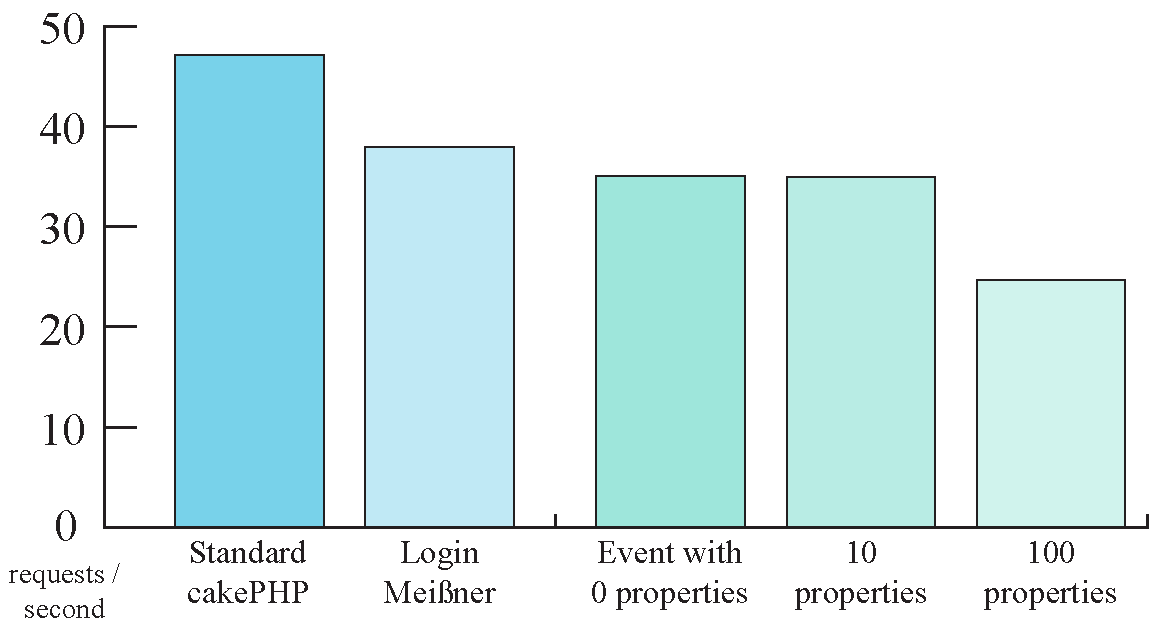
\includegraphics[width=15cm]{fig/ab_result}
	\caption{Benchmark des Webservers mit Apache Bench}
\end{figure}

Die unmodifizierte cakePHP Webanwendung erreicht den Höchstwert 47,14 Anfragen pro Sekunde. Dass hier der höchste Wert vorliegt, war zu erwarten, da das gleiche Framework für die Meißner Anwendung verwendet wurde, allerdings müssen keine Bilder, Skripte, etc. geladen werden.\par

Das Laden der oben genannten Elemente erklärt auch das schlechtere Ergebnis der Meißner App bei der \glqq Login Meißner\grqq{}-Säule. Im Hintergrund werden hier außerdem Skripte von socket.io angefragt, um eine Verbindung zum WebSocket Server aufzubauen. Dadurch ist die App im Allgemeinen komplexer aufgebaut und erreicht so nur einen Wert von 37,95 Anfragen pro Sekunde. Dieses Ergebnis ist für das flüssige Bedienen der Anwendung vollkommen ausreichend und wird in der Praxis durch den Offline Cache weiter beschleunigt, da nicht mehr so viele Requests an den Server gestellt werden müssen.\par

In grün gehalten wird deutlich, wie ein Event mit mehr Details deutlich länger zum Laden benötigt. Dabei sind für die Übersichtsseite zur Bearbeitung einer Veranstaltung widerrum mehr Anfragen notwendig als für die Startseite der Meißner App und erreicht somit einen Wert von 35,04 bearbeiteten Anfragen pro Sekunde.

\newpage
Wenige Eigenschaften sorgen für keinen signifikant schlechteren Wert. So erreicht eine Veranstaltung mit nur 10 Eigenschaften mit 34,92 Anfragen pro Sekunden nahezu den gleichen Wert wie ein leeres Event. Nur bei einer hohen Anzahl wird der Aufruf der Seite komplexer und verlangsamt sich auf 24,67 Anfragen pro Sekunde.

\subsection{Fazit}
Mit erhöhter Komplexität eines Views verlängert sich die Zeit, die der Webserver zum bereitstellen benötigt. Das trifft die Erwartungen und ist auch wenig verwunderlich, da mehr Daten aus der Datenbank erfragt und aufbereitet werden müssen. Alle Ergebnisse sind allerdings gut für einen Server, der auf einem Notebook läuft.\par

Der Server erfährt in der Praxis aber eine geringere Belastung, da der Offline-Cache viele Requests unnötig macht. Denn nur veränderte Dateien werden neu vom Server angefragt, abgesehen von den dynamischen Bibliotheken für socket.io oder Google Maps.

%%%%%%%%%%%%%%%%%%%%%%%%%%%%%%%%%%%%%%%%%%%%%%%%%%

\section{WebSockets mit node.js}
Bei den WebSockets wird analysiert, wie groß die Pakete, die verschickt werden, tatsächlich sind und wie viel Arbeitsspeicher dafür von node benötigt wird.

\subsection{Speicherauslastung}
Zunächst wird versucht zu erfassen, wie viel Arbeitsspeicher pro geöffnetem WebSocket benutzt wird. Das ist interessant, weil es eine messbare Größe ist, die angibt, wie viele WebSockets bei festem Arbeitsspeicher verwaltet werden können.\par

Als Testsystem kommt das gleiche MacBook Pro wie beim Apache2 zum Einsatz, da sowohl Apache als auch node.js auf dem gleichen Server installiert sind.

\newpage
Für den Versuch wird mit dem Tool \emph{Activity Monitor} (integriert in OS X) die Speicherauslastung von node gemessen und so die durchschnittlichen Anforderungen für jede aktive Verbindung ermittelt.

\subsection{Messung der Speicherauslastung}
Es wurden drei Messreihen durchgeführt in denen über den Browser Google Chrome je 50 Sockets geöffnet wurden. Dabei stieg die Speicherauslastung im Schnitt von 75,50 MB auf 78,63 MB an. Die CPU Auslastung betrug dabei ca. 2-3\%. Demnach benötigt eine aktive Verbindung zu node.js ca. 63 KBytes.\par

Somit berechnet sich die zusätzliche Speicherauslastung für 1000 Clients wie folgt:
\begin{align*}
	1.000 \times 63 \mbox{ KBytes} = 63.000 \mbox{ KBytes} \sim 61,5 \mbox{ MB}
\end{align*}
Die Messung gestaltete sich relativ schwierig, da die Garbage Collection von node.js ab und zu Speicher freigab, was einige Messreihen unbrauchbar machte. Es finden also noch weitere eigene Optimierungsvorgänge statt, um den Speicherverbrauch möglichst gering zu halten. Diese werden automatisch von node.js ausgeführt.

\paragraph{Fazit}
Die Tests haben gezeigt, dass die Speicherauslastung durch WebSockets geringer ist, als erwartet wurde. Dadurch können sehr viele Clients bei geringem Speicheranspruch verwaltet werden.

\subsection{Netzwerkauslastung}
In dem Kapitel über die WebSockets wurde beschrieben, dass die Netzwerkauslastung bei eben diesen besonders gering sein soll. Das liegt daran, dass der Header eines WebSockets mit gerade 2 Bytes pro Nachricht auskommt, während bei normalen HTTP Anfragen ein Header von ca. 700-800 Bytes benötigt wird \cite{chromium:headers}.\par

Beim vorgestelltem \emph{Polling} sind diese 700-800 Bytes beim HTTP-Request und HTTP-Response notwendig. Das würde bedeuten, dass bei 1.000 Clients nur für den Header ohne weiteren Inhalt und bei einem Intervall von einer Sekunde folgende Rechnung aufgestellt werden kann:
\begin{align*}
	1.000 \times 800 \ \frac{\mbox{Bytes}}{\mbox{Sekunde}}= 800.000 \ \frac{\mbox{Bytes}}{\mbox{Sekunde}} = 6.400.000 \ \frac{\mbox{Bits}}{\mbox{Sekunde}} \sim 6,104 \mbox{ Mbps}
\end{align*}
Im Vergleich dazu macht sich der deutlich schmalere Header der WebSockets bemerkbar. Auch hier wird zur Vereinfachung von einer sekündlichen Übermittlung einer Nachricht mit 1.000 Clients ausgegangen:
\begin{align*}
	1.000 \times 2 \ \frac{\mbox{Bytes}}{\mbox{Sekunde}}= 2.000 \ \frac{\mbox{Bytes}}{\mbox{Sekunde}} = 16.000 \ \frac{\mbox{Bits}}{\mbox{Sekunde}} \sim 0,015 \mbox{ Mbps}
\end{align*}
Das bedeutet, dass über 400\% Overhead durch WebSockets eingespart werden kann. Da die Meißner App vor allem mobil genutzt werden soll, ist dieses Ersparnis von großer Bedeutung: Umso weniger Daten für die Echtzeitaktualisierung benötigt werden, desto schneller und zuverlässiger können publish-Nachrichten die Endgeräte erreichen.

\paragraph{Komplexität}
Mit jeder Nachricht, die an den WebSocket Server geschickt wird, gibt es eine Antwort, die fast immer eine Broadcast-Nachricht darstellt. Das hat zur Folge, dass auf eine einzige Nachricht $n$ Nachrichten an verbundene Clients folgen. Wenn nun alle $n$ Clients eine Nachricht verschicken, werden $n \times n = n^2$ Antworten vom WS Server versendet. Dadurch ergibt sich eine quadratische Komplexität für diese Implementierung.\par

Für die Anwendung stellt dies ein Problem dar, wenn hinreichend viele Endgeräte gleichzeitig Nachrichten verschicken. Das Verschicken einer neuen Geoposition findet mit jeder Veränderung der Position statt. Auf diese Weise können schnell sehr viele Updates zusammenkommen. Die quadratische Anzahl von Antworten könnte an dieser Stelle zu einer Überlastung des Servers führen.

\newpage
\paragraph{Optimierung: Puffermanagement}
Mit einem intelligenten Puffermanagement könnte das verhindert werden. Es müsste Nachrichten erst puffern und dann den Inhalt nach Aktualität untersuchen. Wenn zum Beispiel in einem Puffer zwei Nachrichten mit neuen Positionen eines Clients sind, so könnte die Nachricht, die zuerst an den WS Server geschickt wurde, verworfen werden, da schon ein weiteres Update auf diese Position folgt.

\paragraph{Optimierung: Intervalle einrichten}
Bei zu hoher Belastung könnten gewisse Intervalle eingerichtet werden, bei denen die Endgeräte die Updates vom Server erhalten. Die Echtzeitaktualisierung wäre etwas eingeschränkt, aber die Belastung des Netzwerkes und des Servers könnten hierdurch deutlich verringert werden.

\paragraph{Skalierung}
Die Anwendung wurde in erster Linie für circa 90 Clients entwickelt. Bei dieser geringen Anzahl werden die Server nicht überfordert sein. Bis zu 50 Clients gleichzeitig wurden erfolgreich getestet und haben node.js nicht besonders gefordert. Durch die quadratische Komplexität ist dies allerdings nicht für beliebige Anzahlen von Endgeräten garantiert. Das kann durch das oben angesprochene intelligente Puffermanagement gelöst werden, wodurch die Anzahl der Nachrichten reduziert wird und somit auch deutlich mehr Clients gleichzeitig Updates oder Chat-Nachrichten verschicken können.








